\begin{pastexam}[label={px:ncku-112-prog-08}]{成大資訊聯招 112 學年度 第 8 題}
（複選）

{[5\%]} Consider an Min-Max heap represented as an array [3, 20, 13, 6, 5, 4, 8, 10, 15, 12, 9, 7]. If
we exchange any two values X and Y in the array, which of the choices is (are) NOT Min-Max heap(s)?
\begin{enumerate}[label=(\Alph*)]
\item 5 and 7
\item 4 and 9
\item 8 and 9
\item 13 and 9
\item 5 and 10
\end{enumerate}
\end{pastexam}

\begin{pastsoln}
答案：(B)(E)。

最小最大堆積（資結書第~8.5~節）：完全二元樹，奇數層（根在第 $1$ 層）是最小層，偶數層是最大層。 最小層的
節點不大於子樹裡的每一個節點，最大層的節點不小於子樹裡的每一個節點。 陣列從 $1$ 開始，位置 $i$ 的子節點在
$2i$、$2i + 1$：
\begin{center}
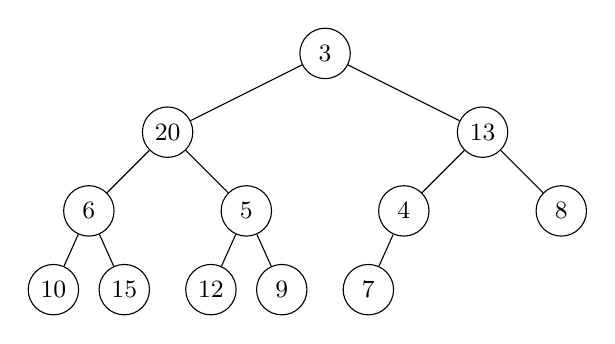
\begin{tikzpicture}[level distance=10mm,
  every node/.style={circle,draw,inner sep=0pt,minimum size=6.4mm,font=\small},
  level 1/.style={sibling distance=40mm}, level 2/.style={sibling distance=20mm},
  level 3/.style={sibling distance=9mm}]
\node {3}
  child {node {20}
    child {node {6} child {node {10}} child {node {15}}}
    child {node {5} child {node {12}} child {node {9}}}}
  child {node {13}
    child {node {4} child {node {7}} child[missing]}
    child {node {8}}};
\end{tikzpicture}
\end{center}
第 $1$ 層（最小）$3$；第 $2$ 層（最大）$20, 13$；第 $3$ 層（最小）$6, 5, 4, 8$；第 $4$ 層（最大）
$10, 15, 12, 9, 7$。 原陣列是合法的：$3$ 是最小值；$20 \ge$ 它子樹的 $6, 5, 10, 15, 12, 9$；$13 \ge 4, 8, 7$；
$6 \le 10, 15$；$5 \le 12, 9$；$4 \le 7$。

交換兩個值只會影響這兩個位置和它們的祖先、子孫之間的關係，逐項只檢查這些：
\begin{itemize}
\item (A) $5$（位置 $5$，最小層）和 $7$（位置 $12$，最大層）。 位置 $5$ 變 $7$：$7 \le$ 子節點 $12, 9$，而
祖先 $20 \ge 7$、$3 \le 7$。 位置 $12$ 變 $5$：父 $4 \le 5$，祖父 $13 \ge 5$，根 $3 \le 5$。 仍是最小最大堆積。
\item (B) $4$（位置 $6$）和 $9$（位置 $11$）。 位置 $6$ 變 $9$，在最小層，但子節點 $7 < 9$；位置 $11$ 變 $4$，
它的父節點 $5$ 在最小層，$5 > 4$。 \textbf{不是}。
\item (C) $8$（位置 $7$）和 $9$（位置 $11$）。 位置 $7$ 變 $9$：沒有子節點，父 $13 \ge 9$，根 $3 \le 9$。 位置
$11$ 變 $8$：父 $5 \le 8$，祖父 $20 \ge 8$。 仍是。
\item (D) $13$（位置 $3$）和 $9$（位置 $11$）。 位置 $3$ 變 $9$，在最大層，子樹是 $4, 8, 7$，都 $\le 9$；位置
$11$ 變 $13$：父 $5 \le 13$，祖父 $20 \ge 13$，根 $3 \le 13$。 仍是。
\item (E) $5$（位置 $5$）和 $10$（位置 $8$）。 位置 $5$ 變 $10$，在最小層，但子節點 $9 < 10$；位置 $8$ 變 $5$，
父節點 $6$ 在最小層，$6 > 5$。 \textbf{不是}。
\end{itemize}
題目問哪些\textbf{不是}最小最大堆積，選 (B)(E)。
\end{pastsoln}
